\subsection{Phonological objects in \CVCV}
\label{subsec:intro:obj}

This section briefly introduces the representation
of different phonological objects in the language of
\CVCV.

\TODO{Reihenfolge}

\TODO{vllt alles eine Hierarchieebene höher $\implies$ flache Hierarchie?}

\subsubsection{Long vowels}
\begin{structure}{}
  \drawCV{1}
  \C{C}
  \longV{V}
\end{structure}
\TODO{complement needs to be licensed}


\subsubsection{Diphtongs}
\TODO{Which structure is correct?

\begin{structure}{\emph{some} Relation}
  \drawCV{1}
  \C{C}
  \V{V\textsubscript{1}}
  \emptyC
  \V{V\textsubscript{2}}
  \draw[dashed] (pV2) -- (V1);
\end{structure}

\begin{structure}{association to 2 Nuclei}
  \drawCV{1}
  \C{C}
  \V{V\textsubscript{1}}
  \emptyC
  \V{V\textsubscript{2}}
  \draw (pV2) -- (V1);
\end{structure}
}


\subsubsection{Coda}\label{intro:obj:coda}
Coda consonants are defined as Onsets that occur before
a governed empty Nucleus.\parencite[p.~192]{scheer2004}
This Nucleus can either be governed by a following full
vowel, \wordunsure{IG} or because it is the final
vowel in the domain.
\Cref{fig:intro:obj:coda} shows the two different kinds
of Codas.
\marknote{2 kinds, but with IG 3 options were mentioned before?!}

\begin{figure}[h]
  \centering
  \begin{subfigure}{.49\textwidth}
    \centering
    \begin{structure}{}
      \drawCV{2}
      \V{V}
      \C{C}
      \C{\bfseries C}
      \emptyV[gov]
      \C{C}
      \V{V}
    \end{structure}
    \caption{internal Coda}
  \end{subfigure}
  \hfill
  \begin{subfigure}{.49\textwidth}
    \centering
    \begin{structure}{}
      \drawCV{1}
      \V{V}
      \C{C}
      \C{\bfseries C}
      \fen
    \end{structure}
    \caption{final Coda}
  \end{subfigure}
  \caption{Codas in \CVCV}
  \label{fig:intro:obj:coda}
\end{figure}
\TODO{hier schon positional strength of Coda/Coda-Mirror einführen?}

\begin{figure}
  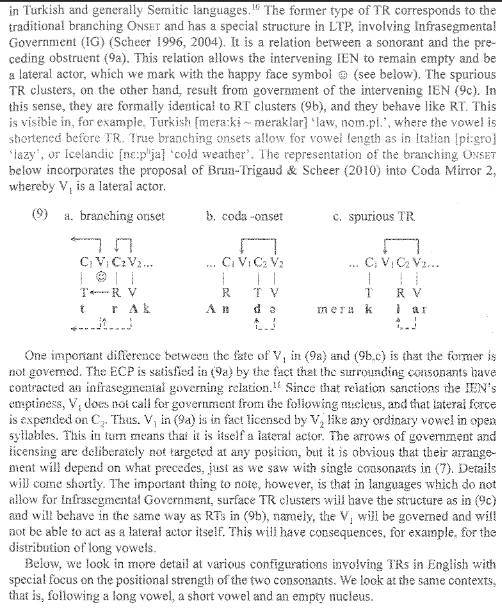
\includegraphics{figures/note_phon_objects_coda_ig.png}
  \caption{from \cite[p.~12]{scheerCyran2017}}
\end{figure}

\subsubsection{(Coda-Mirror) <- unten verwendet? Sonst nur brief mention}
\TODO{}

\subsubsection{Margin contexts:}
\subsubsection{Word-start \ctx{\#\_}}\label{intro:obj:word start}
\begin{structure}{}
  \drawCV{0}
  \wordstart

  \C{C}
  \V{V}
\end{structure}
\TODO{}

\subsubsection{Word-end \ctx{\_\#}}\label{intro:obj:word end}
\TODO{}

\subsubsection{Syllabic consonants}
\TODO{}

\subsubsection{Branching Onsets (Infrasegmental Government)}
\TODO{}

\subsubsection{Vowel-Zero-Alternations}
\TODO{}